\documentclass[titlepage,10pt]{article}
\usepackage{textcomp}
\usepackage{latexsym}
\usepackage{graphicx}
\usepackage{amsmath}
\usepackage{moreverb}
\def\urltilda{\kern -.15em\lower .7ex\hbox{\~{}}\kern .04em}


\begin{document}
\title{
DRAFT: SWIFT Stability Derivatives and Dynamic Analysis\\
}

\author{Zouhair Mahboubi}

\date{December 5$^{th}$, 2009\\ Stanford University}

\maketitle

\tableofcontents
\newpage
\section{Introduction}
In this report, we summarize the approach use to derive the stability and control derivatives for the Swift UAV. We use two methods and cross-compare the results. Overall, we find good agreement between the two approaches which bolsters our confidence in them. The complete results and input files are given in the appendix.

\section{Nomenclature and Axes}
In this report we try to use the same notation and axes used in \cite{Etkin}. The non-dimensional coefficients are also the same as those given in Table 4.1 of \cite{Etkin}. All derivatives are by respect to radians unless otherwise stated. As for the reference geometry, we use the following values for surface area, span and M.A.C. These differ slightly from the Swift values due to simplifications in the model. However, we were consistent in using the same reference values in both LinAir and XFLR5 models. 
\begin{itemize}
\item M = 150 kg = 330 lbs
\item $x_{CG}$ = 1.2 m behind Leading Edge of Wing
\item S = 12.1 m = 39.4 ft
\item b = 13.1 $m^2$ = 141 $ft^2$
\item $\bar{c}$ = 1.06 m = 3.47 ft
\end{itemize}

\section{Analysis}
\subsection{2D section computations}
Using the 3D CAD representation of the Swift airplane, we extracted 5 representative airfoil sections that we have used for analysis. Four of the sections were chosen at the control surface breaks in the spanwise direction for convenience, and the 5th one mid-span of the winglet.\\

We then used XFLR5 (a gui-interface for Xfoil, among other things) to compute the drag polars for the sections. These computations assumed viscous flow \footnote{Xfoil uses the Integral Boundary Layer method}, with Ncrit=13 (sailplane) and forced transition at 25\% of the chord (the Swift has a transition tape on its surface) and were done for a range of Reynolds Numbers. We also carried computations with the flaps deflected at different angles in order to find the effect on the section lift-coefficient, drag-coefficient and aerodynamic moment.

\begin{figure}[bht]
\begin{center}
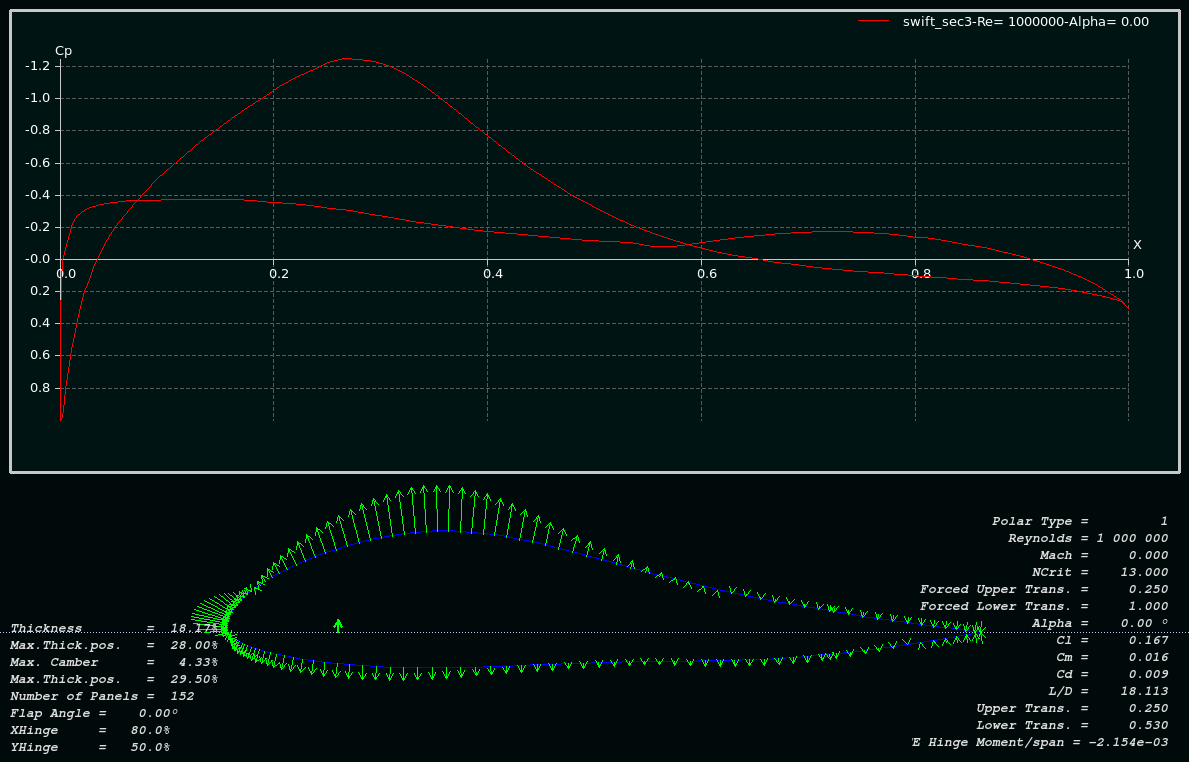
\includegraphics[width = 100mm]{xfoil_section.png}
\end{center}
\caption{Sample Result from 2D section using XFoil}
\label{xfoil}
\end{figure}

\subsubsection{Hinge Moments}
In order to size the actuators, hinge moments computations we necessary. Again, using Xfoil we computed the maximum expected hinge-moment coefficients. These were obtained by using up to $40^o$ deflections for the flaps and $20^o$ for the ailevons at angle of attacks past-stall (From \cite{NACA9} "Airfoil stall is accompanied by a rapid increase in hinge-moment coefficient. Air-flow separation over the flaps causes the hinge moment curves to become non linear and sometimes to reverse slop"). Using the surface area for each section, we converted these to moments using the worst case scenario of flying at the $V_{ne}=120km/h$. It's worth mentioning that XFoil's hinge moments are normalized by respect to the Wing's chord $Hm = C_h\ q\  b_{flap}\ c_{airfoil}^2$ rather than flap chord as done in \cite{Etkin} $Hm = C_h\ q\ b_{flap}\ c_{flap}^2$. Using the correct coefficient, results were in good agreement with those computed using full CFD analysis as showed by the following table. The difference in results for ailevons is due to the fact that the CFD model used $30^o$ deflections rather than $20^o$

\begin{table}[h]
\begin{center}
\begin{tabular}{|l | c | c | c| c|}
\hline
	Xfoil Results & Inner Flap & Outter Flap & Inner Ailevon & Outter Ailevon\\
\hline
Ch &0.46&	0.46	&0.2	&0.2\\
Hinge-moment (lbs) & 29.33	&16.55	&11.12&	7.92\\
Actuator Force (lbs)& 70.39	&39.72	&44.49&	31.70\\
\hline
\hline
	CFD Results &  & & & \\
\hline
Ch & 0.376&	0.395	&0.381	&0.410	\\		
Hinge-moment (lbs) & 24.23&	14.36	&21.19&	16.25\\
Actuator Force (lbs)& 58.15&	34.47&	84.74	&65.02 \\
\hline
\end{tabular}
\end{center}
\end{table}

			

\subsection{3D Computations}
\subsubsection{LinAir Method}
We model the aircraft in LinAir, which solves an irrotational, inviscid, linearized flow around the airplane. The model we use is simplified in that we only make use of the root and tip sections. LinAir has the option of specifying 2D section properties, so we use the results obtained by XFoil at a representative Reynolds Number. Unfortunately handling control derivatives is not easy in LinAir. The following table summarizes the derivatives, The input file is given in the appendix. Note that although LinAir reports the linearized drag-coefficient derivative around the current AoA, $CD$ is not linear in AoA (i.e. $CD_{\alpha}$ is a strong function of $\alpha$).

\begin{table}[h]
\begin{center}
\begin{tabular}{|l | c | c | c| c| c| c|}
\hline
Derivatives	&CL&      		CD      	&Cm      	&Cy    &  	Cn      &	Croll   \\
@$\alpha=-1.5$	&0.59			&0.023          &-0.005         &0.0    &       0.0     &   0.0 \\
\hline
Alpha   	&4.9998&		0.2624&		-0.7124&	0.0000&		0.0000&		0.0000\\
Mach    	&0.0473&		0.0026&		-0.0028&	0.0000&		0.0000&		0.0000\\
$\hat{q} $  	&6.2151&		0.2421&		-3.1388&	0.0000&		0.0000&		0.0000\\
\hline
Beta    	&0.0000&		0.0000&		0.0000&		-0.4297&	0.04690&	-0.1332\\
$\hat{p}$   	&0.0000&		0.0000&		0.0000&		-0.1806&	-0.0027&	-0.6296\\
$\hat{r}  $ 	&0.0000&		0.0000&		0.0000&		0.19370&	-0.0302&	0.16355\\
\hline
\end{tabular}
\end{center}
\caption{LinAir Derivatives}
\end{table}

\begin{figure}[hb]
\begin{center}
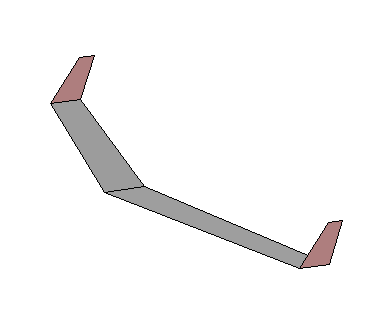
\includegraphics[height = 70mm]{LinAir.png}
\end{center}
\caption{LinAir Geometry Snapshot}
\label{linair}
\end{figure}
\clearpage

\subsubsection{XFLR5 Method}
XFLR5 also has an implementation of a Vortex-Lattice method similar to LinAir, but because it's able to compute the 2D section properties using Xfoil, it's relatively straightforward to add more spanwise 2D sections. Moreover, it is easy to deflect a section's trailing edge to model flap or ailevon deflections. However, the disadvantage is that it does not directly give the stability and control derivatives, nor does it handle roll, pitch and yaw rates (p, q and r) while LinAir does.\\

So our approach was to generate look-up tables of lift, drag and side force coefficients as well as pitch, roll and yaw moment coefficients. We then imported the data in Matlab, and assuming linear behaviour when appropriate (quadratic for drag) we used least-squares to approximate the derivatives. Let's take the lift-coefficient as an example, we know that in general $$CL = CL_0 + CL_{\alpha} \alpha + CL_{\delta_{f}}\ \delta_f$$ So if we have a look-up from $\alpha$ and $\delta_f$ to $CL$, we can write this in vector form: $$\left[CL\right]_i =  \left[1\ \alpha_i\  (\delta_f)_i  \right] \left[ CL_0\ CL_{\alpha}\ CL_{\delta_{f}}\right]^T$$ If we stack all of the $\left[1\ \alpha_i\  (\delta_f)_i\  \right]$ in a matrix, it is then possible to use least-squares to estimate the $\left[ CL_0\ CL_{\alpha}\ CL_{\delta_{f}}\right]$. A similar approach can be done for pitching moment, rolling moment, etc. It's worth mentioning that we assume longitudinal and lateral coefficients are decoupled (i.e. Rolling moment only depends on ailevon deflections and side-slip, and not angle of attack or flap deflections). Given that the vortex-lattice method is linear, we expect that linearizing the data should yield good results, and plots included in the appendix confirm this. The Matlab script used to extract these coefficients is also included in the appendix.\\

Table \ref{table:XFLR5} summarizes some of the derivatives we extracted from the XFLR5 data. Flaps deflection downawrd is taken to be positive while positive ailevon deflections is taken to be such as positive rolling moment is produced (i.e. left ailevon down and right ailevon up). We have omitted the drag coefficient since it's not linear in AoA nor flap deflections over the entire range of AoA. If computation power for simulations is not an issue, we recommend using look-up tables. For analysis, we need to linearize it around trim conditions. It is also worth mentioning that all computations were only done up to beginning of stall. So if derivatives are used instead of look-up tables, one must be careful not to exceed the alpha limits, which actually depend on flap deflections (flaps increase lift-coefficient but decrease maximum AoA)

\begin{table}[h]
\begin{center}
\begin{tabular}{|l | c | c | c| c| c|}
\hline
Derivatives	&CL      		&Cm      	&Cy    &  	Cn      &	Croll   \\
@$\alpha=0$  &0.6044			&0.0077         &0.0    &       0.0     &   0.0 \\
\hline
Alpha 		 &4.8594		&-0.6834      & -  &  - &  - \\
$\delta_{flap1}$ &0.7795		&0.0817      & -  &  - &  - \\
$\delta_{flap2}$ &0.5170		&-0.1039      & -  &  - &  - \\
\hline
Beta		 & - 		        &-	      & -0.3012  &  0.0031 &  -0.1322 \\
$\delta_{ailevon1}$ & - 	        &-	      & 0.0223 &  -0.0070 &  0.1999 \\
$\delta_{ailevon1}$ & - 	        &-	      & 0.0860 &  -0.0050 &  0.2078 \\
\hline
\end{tabular}
\end{center}
\caption{XFLR5 Derivatives}
\label{table:XFLR5}
\end{table}



\begin{figure}[hb]
\begin{center}
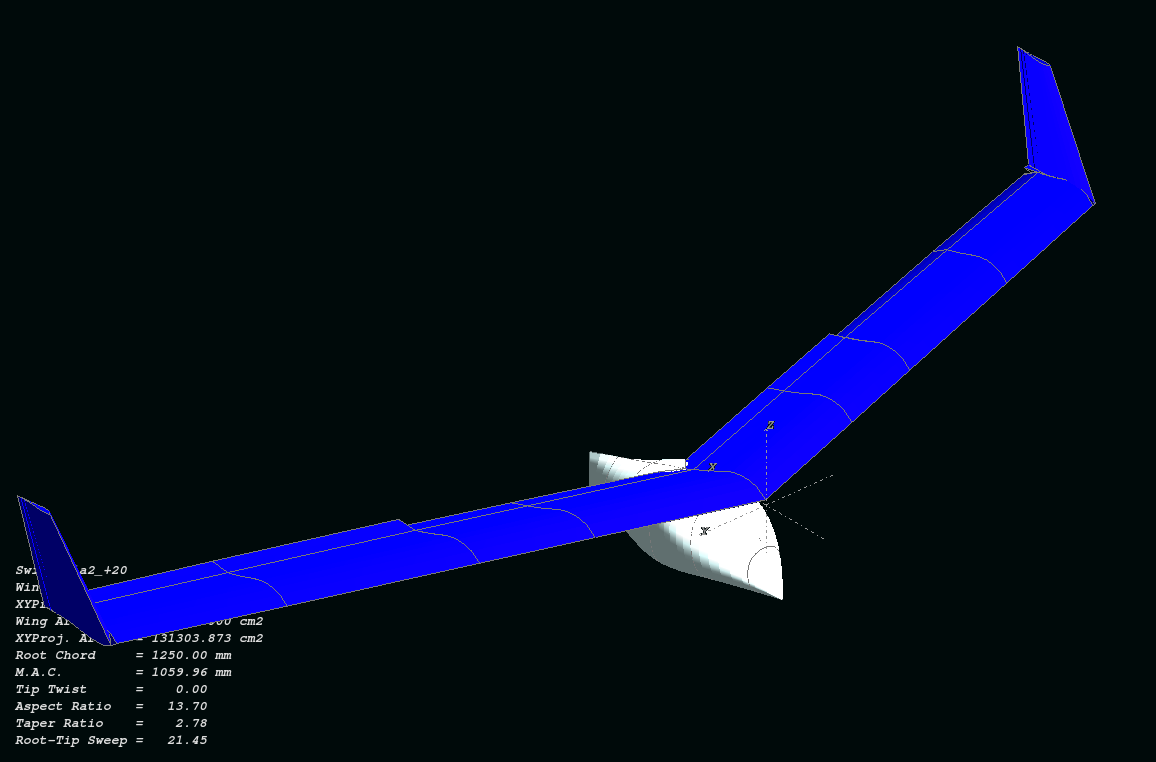
\includegraphics[height = 80mm]{xflr5.png}
\end{center}
\caption{XFLR5 Geometry Snapshot (deflected ailevons)}
\label{xflr}
\end{figure}



\clearpage
\subsubsection{Comparison of methods}
As mentioned earlier, reference areas and lengths were chosen to match between the two models in order to facilitate comparison. Moreover, the point around which we linearize the data was chosen so that the lift coefficient matches (AoA of $0$ in XFLR5 model and $-1.5$ in LinAir). Table \ref{table:comp} lists the results of the two methods next to each other.

\begin{table}[h]
\begin{center}
\begin{tabular}{|l | c | c | c | c| c|| c| c| c| }
\hline
Quantity &  $\alpha$ &$CD$ & $CL$ & $CL_{\alpha}$  &  $Cm_{\alpha}$ &  $Cy_{\beta}$ &  $Cn_{\beta}$  & $Cl_{\beta}$ \\
\hline
Linair   &  -1.5     &0.023  & 0.60  &  4.99   	   &   -0.71        &  -0.43        &  0.0031        & -0.1332  \\
XFLR5    &  0        &0.022  & 0.59  &  4.86       &   -0.68        &  -0.30        &  0.0469        & -0.1322  \\
\hline
\end{tabular}
\caption{LinAir - XFLR5 Comparisons}
\label{table:comp}
\end{center}
\end{table}

Clearly all the quantities match quite well, apart from the yawing moment. This turns out to be a limitation in XFLR5's implementation, and a report comparing calculations and experimental results concluded 'Yawing moment predictions give the correct trend - no more' \cite{XFLR5exp}\\

Based on this comparison of results, we are left with the decision to choose between one of the models. LinAir provides us with the rate derivatives and does better in predicting yawing moment, but it uses a more simplified model and makes it hard to extract control derivatives. On the other hand, XFLR5 uses more spanwise sections with their drag polars, allows us to extract control derivatives but does not give rate derivatives and underpredicts the yawing moment. So rather than chose one of the models, we make the decision to use both: Given that the results are overall in good agreement, mixing both models should yield good results.\\

Our approach will be to use the look-up tables produced by XFLR5 for simulations and LinAir for dynamic analysis. The reason for this is that the look-up tables provide a simple way to account for non-linear effects (quadratic drag, forces due to control deflections and stall-limits), while the LinAir stability derivatives -augmented with the control derivatives- provide a simple way to linearize the model around an operating point and extract a state-space representation which can be used for control analysis and design.

\textbf{Still need to find a concise way to represent $CD$ as a function of $CD_0$ $CD_\alpha$ or $CD_{CL}$, $CD_{f1}$, , etc. }


\section{Dynamic Analysis - Work in Progress ....}
Given the stability derivatives, construct the A and B matrices ...
LinAir is capable of giving the roots (i.e. eigen values) but we want the zeros as well if we want to control
So far, all of this has been dimensionless, We know need to start talking about 'operating points', more urgently
we need more accurate estimates MOMENTS OF INERTIA!!!


 								 
\section{Conclusion}
We used Xfoil to find 2D section properties for the Swift Uav, which was modeled in two vortex-lattice programs: LinAir and XFLR5. We compared the results of the two methods and found overall good agreement, which encouraged us in combining the results to obtain the complete stability and control derivatives for the airplane. ... more work to be done to find the state-space representation of the airplane!


\begin{thebibliography}{9}
\bibitem{Etkin}
  Etkin B. Reid L.,
  Dynamics of Flight: Stability and Control.
  3rd Edition.
  1996.
  
\bibitem{NACA9}
 M. L. Spearman,
 Wind-tunnel investigation of control surface characteristics on NACA 0009 airfoil.
 Technical Note NACA-WR-L-47
 November 1947

\bibitem{XFLR5exp}
  A. Deperrois,
  Comparison of Experimental Data to XFLR5 Results.
  http://xflr5.sourceforge.net/xflr5.htm
  [Retrieved November 2009]


\end{thebibliography}
\newpage
\appendix

\newpage
\section{XFLR5 look-up tables}
The following tables represent look-up tables for the Swift UAV in different configurations as a function of AoA. The last AoA given represents the limit of stall, and anything after it the wing has stalled (i.e. large increase in drag and drop in lift coefficient). The runs were done at constant lift by varying Qinf, so the 'freestream speed' line is not used. \\

It should be possible to interpolate between tables if done with care. Per example, to find the lift coefficient with $10^o$ of $\delta_{f1}$ and $-5^o$ of $\delta_{f2}$, we would interpolate tables A.2 and A.5 relative to the zero-flap deflection case (A.1) to find the contribution of each flap to the increment in lift, then sum the two increments and add the contributions together. Although this is in a way already done when we extract the control derivatives.

\textbf{It is important to remember that the Yawing Moment given by XFLR5 is not to be trusted. We recommend using the $Cn$ coefficients given by LinAir instead}

\subsection{$\delta_{f1} = 0$ , $\delta_{f2} = 0$ , $\delta_{a1} = 0$, $\delta_{a2} = 0$ , $\beta=0$ (f1f2\_0)}
\begin{tiny}\verbatimtabinput[2]{../data/f1f2_0.txt}\end{tiny}

\subsection{$\delta_{f1} = -20^o$ , $\delta_{f2} = 0$ , $\delta_{a1} = 0$, $\delta_{a2} = 0$ , $\beta=0$ (f1\_-20)}
\begin{tiny}\verbatimtabinput[2]{../data/f1_-20.txt}\end{tiny}

\subsection{$\delta_{f1} = +20^o$ , $\delta_{f2} = 0$ , $\delta_{a1} = 0$, $\delta_{a2} = 0$ , $\beta=0$ (f1\_+20)}
\begin{tiny}\verbatimtabinput[2]{../data/f1_+20.txt}\end{tiny}

\subsection{$\delta_{f1} = +30^o$ , $\delta_{f2} = 0$ , $\delta_{a1} = 0$, $\delta_{a2} = 0$ , $\beta=0$ (f1\_+30)}
\begin{tiny}\verbatimtabinput[2]{../data/f1_+30.txt}\end{tiny}

\subsection{$\delta_{f1} = 0$ , $\delta_{f2} = -20^o$ , $\delta_{a1} = 0$, $\delta_{a2} = 0$ , $\beta=0$ (f2\_-20)}
\begin{tiny}\verbatimtabinput[2]{../data/f2_-20.txt}\end{tiny}

\subsection{$\delta_{f1} = 0$ , $\delta_{f2} = +20^o$ , $\delta_{a1} = 0$, $\delta_{a2} = 0$ , $\beta=0$ (f2\_+20)}
\begin{tiny}\verbatimtabinput[2]{../data/f2_+20.txt}\end{tiny}

\subsection{$\delta_{f1} = 0$ , $\delta_{f2} = +30^o$ , $\delta_{a1} = 0$, $\delta_{a2} = 0$ , $\beta=0$ (f2_+30)}
\begin{tiny}\verbatimtabinput[2]{../data/f2_+30.txt}\end{tiny}

\subsection{$\delta_{f1} = 0$ , $\delta_{f2} = 0$ , $\delta_{a1} = +20^o$, $\delta_{a2} = 0$ , $\beta=0$ (a1\_+20)}
\begin{tiny}\verbatimtabinput[2]{../data/a1_+20.txt}\end{tiny}

\subsection{$\delta_{f1} = 0$ , $\delta_{f2} = 0$ , $\delta_{a1} = 0$, $\delta_{a2} = +20^o$ , $\beta=0$ (a2\_+20)}
\begin{tiny}\verbatimtabinput[2]{../data/a2_+20.txt}\end{tiny}

\subsection{$\delta_{f1} = 0$ , $\delta_{f2} = 0$ , $\delta_{a1} = 0$, $\delta_{a2} = 0$ , $\beta=-4^o$  (beta\_4)}
\begin{tiny}\verbatimtabinput[2]{../data/beta_4.txt}\end{tiny}

\subsection{$\delta_{f1} = 0$ , $\delta_{f2} = 0$ , $\delta_{a1} = 0$, $\delta_{a2} = 0$ , $\beta=-8^o$  (beta\_8)}
\begin{tiny}\verbatimtabinput[2]{../data/beta_8.txt}\end{tiny}

\newpage
\section{Matlab script for XFLR5 data}
\subsection{Comparison of Linearized data with Look-up tables}
The following three graphs show lift-coefficient, pitching-moment and rolling-moments as a function of AoA for different flap and ailevon settings. The solid lines represent the data from XFLR5 while the 'x' points are the values interpolated using the derivatives extracted from the Matlab script.

\begin{figure}[hb]
\begin{center}
\begin{tabular}{cc}

\includegraphics[height = 50mm]{../data/cl.png} & \includegraphics[height = 50mm]{../data/cm.png} \\
\includegraphics[height = 50mm]{../data/rm.png} & \includegraphics[height = 50mm]{../data/ym.png} \\
\end{tabular}
\end{center}
\caption{XFLR5 coefficients compared to results from derivative extraction}
\end{figure}
\clearpage

\begin{footnotesize}\verbatimtabinput[8]{../data/find_derivatives.m}\end{footnotesize}

\newpage
\section{LinAir Input File and Results}
Incomplete without moments of inertia ...
%\begin{tiny}\verbatimtabinput[2]{Swift.xml}\end{tiny}


\end{document}
